\documentclass{amsart}
\usepackage{master}
\begin{document}
\title{L-spaces, foliations, and left-orderability}
\author{Lecture by Jonathan Hanselman\\
Notes by Jackson Van Dyke}
\thanks{All errors introduced are my own.}
\date{June 19, 2018}
\maketitle

The broad question being driven at here, is what sophisticated symplectic 
notions can tell us about more familiar notions on $3$-manifolds.
Are there any relationships between Heegard Floer (or monopole Floer) homology
and more classical invariants of low-dimensional topology?

\section{$L$-space conjecture}

An $L$-space is, roughly-speaking, is
a $3$-manifold with minimal Heegard Floer homology.
Recall that Heegard Floer homology and monopole Floer homology
are isomorphic.

The so-called $L$-space conjecture is as follows:

\begin{con}
Suppose $Y$ is an irreducible $3$-manifold which is closed and oriented. 
Also suppose $Y$ is a rational homology sphere.
Then TFAE:
\begin{enumerate}
\item $Y$ is not an $L$-space
\item $Y$ has a coorientable taut foliation
\item $\pi_1\left( Y \right)$ is left orderable
\end{enumerate}
\end{con}

We will see what these things actually mean in turn.
If we have a closed orientable $3$-manifold $Y$, 
then we pick a Heegard diagram $\cH$, which is a genus $g$ surface $\Sigma$ paired
with $\vec{\al} = \al_1 , \cdots , \al_g$ and $\al{\b} = \b_1 , \cdots , \b_g$.
Now from this we can define the
chain complex $\hatt{\CF}\left( \cH \right)$,
and then taking homology, we get $\hatt{\HF}\left( Y \right)$.
Recall that $\hatt{\CF}$ is generated by $g$-tuples of intersection
points $\vec{x} = \left( x_1 , \cdots ,x_g \right)$ where
$x_i \in \al_i \cap \b_{\sigma\left( i \right)}$ for some permutation $\sigma$. 

$\hatt{\CF}$ carries a $\ZZ  /2\ZZ$ grading.
We only consider this as a relative grading so we don't have to worry about signs.
We orient each $\al_i$ and $\b_i$, and now each of our intersection points has a sign,
and the grading of each intersection point $\vec{x}$ is given by
\begin{equation}
\gr\left( \vec{x} \right) = 
\prod_{i = 1}^g \sign\left( x_i \right)
\sign\left( \sigma \right)
\end{equation}

\begin{exr}
Let $M$ be the matrix whose $ij$ entry is 
the intersection number of $\al_i$ and $\b_j$ counted with sign. Show:
\begin{qenum}
\item $\abs{\det M} = \abs{\chi\left( \hatt{\CF} \right)} =
\abs{\chi\left( \hatt{\HF}\left( Y \right) \right)}$
\item 
$\abs{\det M} = 
\begin{cases}
\abs{H_1\left( Y, \ZZ \right)} 
& Y \text{ is } \QQ HS^3\\
0 & \text{ o/w }
\end{cases}
$
\end{qenum}
\end{exr}

\begin{cor}
$\rank \hatt{\HF}\left( Y \right) \geq \chi\left( \hatt{\HF}\left( Y \right) \right) = 
\abs{H_1\left( Y , \ZZ \right)}$ if $Y$ is a $\QQ$ homology sphere.
\end{cor}

\begin{defn}
An \emph{$L$-space} is a $3$-manifold such that
\begin{equation}
\rank \hatt{\HF}\left( Y \right)= \abs{H_1\left( Y , \ZZ \right)}
\end{equation}
\end{defn}

Recall that we have the splitting
\begin{equation}
\hatt{\HF} = 
\bdsum_{\fs\in \spin^c\left( Y \right)} 
\hatt{\HF}\left( Y , \fs \right)
\end{equation}
$\spin^c \left( Y \right)$ is affine copy of $H^2\left( Y \right) - H_1\left( Y \right)$. 

\begin{prop}
For $Y$ a $\QQ HS^3$, we have $\rank \hatt{\HF}\left( Y , \fs \right)\neq 0$
for any $\fs$.
\end{prop}

This leads us to another equivalent definition:

\begin{thm}
$Y$ is an $L$-space iff
$\rank \hatt{\HF}\left( Y , \fs \right) = 1$
for all $\fs\in \spin^c\left( Y \right)$.
\end{thm}

\begin{exm}
Consider the lens space $Y = L\left( p , q \right)$.
This is obtained by gluing two solid tori together, and then
you can take this gluing to be the Heegard decomposition.
\begin{figure}
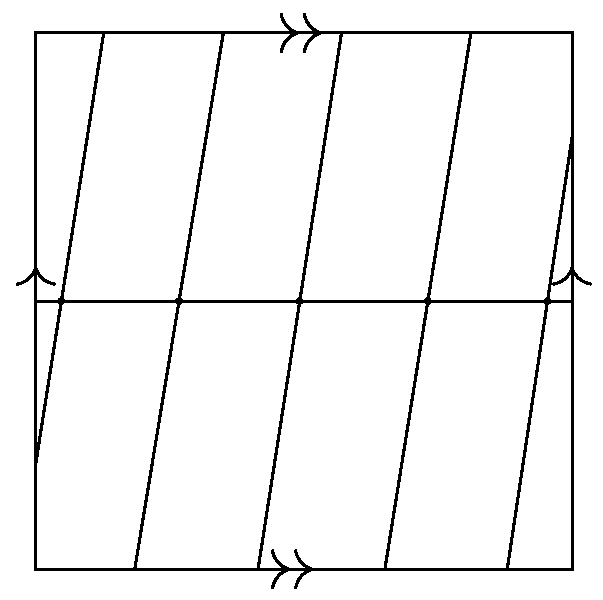
\includegraphics[width=0.4\textwidth]{lens_space.pdf}
\end{figure}
Note there are no holomorphic disks between any generators.
In fact, there are no disks at all. For any pair, there's an obstruction in 
$H_1\left( \Sigma \right) / \lr{\al , \b}\simeqq H_1\left( Y  \right)$ which can
be identified with $\spin^c\left( Y \right)$. 
This tells us that every generator lives in a different $\spin^c$ structure, so $Y$ is
an $L$-space.
\end{exm}

\begin{exm}
Any $Y^3$ with spherical geometry.
This includes lens spaces of course. 
The branched double covers of nonsplit alternating links is always an $L$ space. 
Surgeries on certain knots also yield $L$-spaces. 
For example, $1/1$ surgery on the trefoil yields an $L$-space, and then for any $p / q \geq 1$
yields an $L$-space as well.
\end{exm}

Recall on the chain complex level
\begin{equation}
0\fromto \CF^- \lfromto{i} \CF^\infty \lfromto{\pi} \CF^+\fromto 0
\end{equation}
and on the homology level we get a long exact sequence:
\begin{equation}
\begin{tikzcd}
\cdots \arrow{r}{\dd_-}&
\HF^-\left( Y , \fs \right)\arrow{r}{i_*}&
\HF^{\infty}\left( Y , \fs \right)\arrow{r}{\pi_*}&
\HF^+\left( Y , \fs \right)\arrow{r}{\dd_+}&
\cdots
\end{tikzcd}
\end{equation}
Now we define
the reduced Floer homology:
\begin{equation}
\HF^+_\red\left( Y , s \right)  = \coker \pi_* \simeqq \ker i_* = 
\HF_\red^-\left( Y , s \right)
\end{equation}
This gives us a third equivalent definition of al $L$-space:
\begin{thm}
A $\QQ HS^3$ is an $L$-space iff
$\HF_\red\left( Y \right) = 0$.
\end{thm}

\section{Taut foliations}

Suppose $Y$ is a $3$-manifold, then a cooriented foliation $\cF$ of $Y$ is
a decomposition into oriented surfaces, called leaves, which locally looks like 
\begin{equation}
\RR^3 = \bdun_{z\in R} \RR^2 \times \left\{ z \right\}
\end{equation}

\begin{thm}[Lickorish,Novikov-Zieschang]
Every $3$-manifold has a foliation.
\end{thm}

\begin{exm}
Consider $Y = F\times S^1$. 
Then the foliation can just be
\begin{equation}
\cF = \bdun_{\theta\in S^1} F\times \left\{ \theta \right\}
\end{equation}
\end{exm}

\begin{exm}
$S^3$, or any lens space, has a foliation with only one closed leaf $S^1\times S^1$. 
Each solid torus is foliated as follows:
\begin{figure}
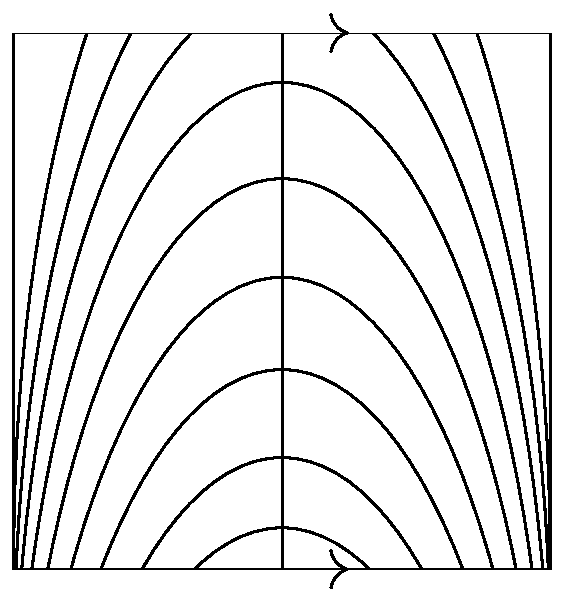
\includegraphics[width=0.4\textwidth]{reeb.pdf}
\caption{The Reeb foliation of $D^2\times S^1$.}
\label{fig:reeb_foliation}
\end{figure}
If this is part of a bigger foliation, it is called a Reeb component.
\end{exm}

We now consider foliations with certain properties.

\begin{defn}
A foliation is \emph{taut} if for every leaf $L$, 
there is a closed curve that is transverse to the foliation, so it intersects every leaf transversely,
intersecting $L$.
\end{defn}

\begin{thm}
Let $\cF$ be a foliation. Then TFAE
\begin{enumerate}
\item A foliation is taut.
\item There is a single transverse closed curve intersecting every leaf.
\item There exists a Riemannian metric such that all of the leaves are minimal surface.
\end{enumerate}
\end{thm}

\begin{prop}
If $\cF$ has a Reeb component, then it is not taut.
\end{prop}

\begin{thm}[Novikov]
If we have a Reebless foliation, then $\pi_1\left( Y \right)$ is infinite
and $Y$ is irreducible. 
\end{thm}

\begin{thm}[Gabai]
If $Y$ is irreducible, and not a $\QQ HS^3$, 
then $Y$ has a taut foliation, which is in particular Reebless.
\end{thm}

\section{Connection to Floer homology}

\begin{thm}[Ozsw\'ath, Zab\'o]
If $Y$ has coorientable taut foliation (CTF) then $Y$ is not an $L$-space. 
\end{thm}

\begin{proof}[Sketch of proof]
Eliashberg-Thurston showed that a CTF can be perturbed in a sufficiently nice way
to a weakly symplectically, semi-fillable
contact structure.
This roughly means we can cap it off
as the boundary of a $4$-manifold with a symplectic structure.
Eliashberg also showed that a symplectic filling of this type can in fact be embedded 
in a closed symplectic $4$-manifold,
so we can sort of cap it off on the other side too, as in \cref{fig:split}.
\begin{figure}
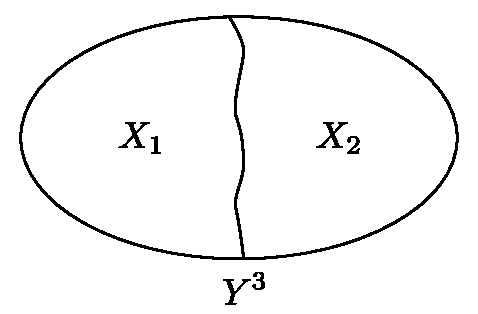
\includegraphics[width=0.3\textwidth]{split.pdf}
\label{fig:split}
\end{figure}
We know that the SW invariant for a $4$-manifold is nontrivial, but we also know about these
relative SW invariants of $X_1$ and $X_2$, but we know that these live in the 
reduced monopole Floer homology
$\HF_\red\left( Y \right)$, which is nonzero, so this is not an $L$-space.
\end{proof}

\section{Left-orderability}

\begin{defn}
A nontrivial group $G$ is left orderable (LO) if
there is a strict total order $<$ such that $g < h$ 
implies $fg < fh$ for all $f\in G$.
\end{defn}

\begin{wrn}
We have made a point to say nontrivial, and by usual convention, 
the trivial group is not considered to be LO.
This is because it makes a lot of other statements cleaner.
\end{wrn}

\begin{exm}
Any finite group is not LO.
More generally, if $G$ has any torsion at all, then $G$ 
is not left-orderable.
\end{exm}

There is maybe no reason to see connections between these things and Floer theory, 
however we do have that

\begin{prop}
If $\pi_1\left( Y \right)$ is finite, then $\pi_1\left( Y \right)$ is not LO.
Also, this being finite implies that that
$Y$ has spherical geometry which, as we saw earlier, are $L$-spaces.
\end{prop}

\begin{prop}
The branch double cover (BDC) of a nonsplit alternating link implies that 
$\pi\left( Y \right)$ is not LO.
\end{prop}

\section{Recent developments}

We know the conjecture holds for Seifert fibered spaces.
This is due to Lisca-Stipsicz for the case of things which are Seifert 
fibered over orientable base-orbifolds.
Bayer-Gordon-Watson checked the nonorientable case.

This is now know to be true for graph manifolds. 
This is based heavily on work of Boyer-Clay.
This has also been shown for cyclic branch covers of knots and links.
We also know exactly when surgeries on knots are $L$-spaces, so this is 
more well understood for this case.
Nathan Dunfield has made extensive computational checks in the process of 
searching for a counterexample.

\end{document}
